\subsubsection*{I.9.2}
\begin{figure}[H]
	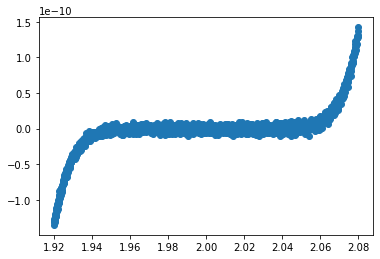
\includegraphics[width=0.5\textwidth]{parts/img/I_9_2_1.png}
	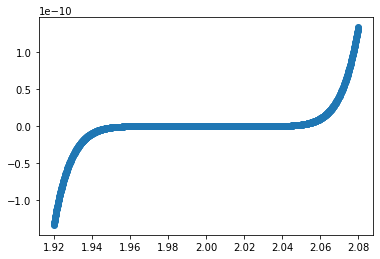
\includegraphics[width=0.5\textwidth]{parts/img/I_9_2_2.png}
\end{figure}
График слева демонстрирует подсчет Горнером, метод справа --- вычислением функции в точке. Горнер плох для вычисления нуля, потому что идет много операций (сложения, умножения) на величинах, порядка $\varepsilon$, из-за чего резко теряется точность вычисления значения, что не дает определить нуль функции. (В отличии от вычисления напрямую, где нам дается нуль с большой точностью)